\chapter{High Frequency Trading}

High frequency trading (HFT) strategies are based on buy and sell assets in
short periods of time gaining a small profit in every transaction, the key is
the amount of transactions that algorithms are capable to execute. 
In 2012 more than 50\% of US market share of exchange trades were HFT.  HFT has
motivated computer-driven strategies capable of processing large amount of data
in short periods of time. 


\section{High Frequency Trading}

HFT is not a strategy but a technology which allow to implement particular
trading strategies. The aim of HFT is to benefit from market short-term pricing
inefficiencies~\cite{chlistalla2011}. HFT is characterized for the use of
high-speed and sophisticated quantitative and algorithmic computer applications
for modeling and executing orders efficiently. In order to make fast decisions,
HFT firms require speed access to trading center servers and sometimes they are
physically near minimizing network latencies.

High frequency trades are short-term positions that commonly end the trading
day avoiding leaving opened positions to the next business day. HFT is
frequently associate to Algorithm trading strategies, but the former is focused
in to reduce the market impact of large institutionals positions.
Figure~\ref{fig:HFTtimes} shows a survey done to traders about the holding time
of a position opened. Most of them agreed that HFT refers to positions between
1-second and 10-minutes. Overnight positions are avoided since they are more
risky and also more expensives fees, HFT firms end the trading day closing all
opened positions.



\begin{figure}[!h]
  %\vspace{-0.8cm}
  \centering
  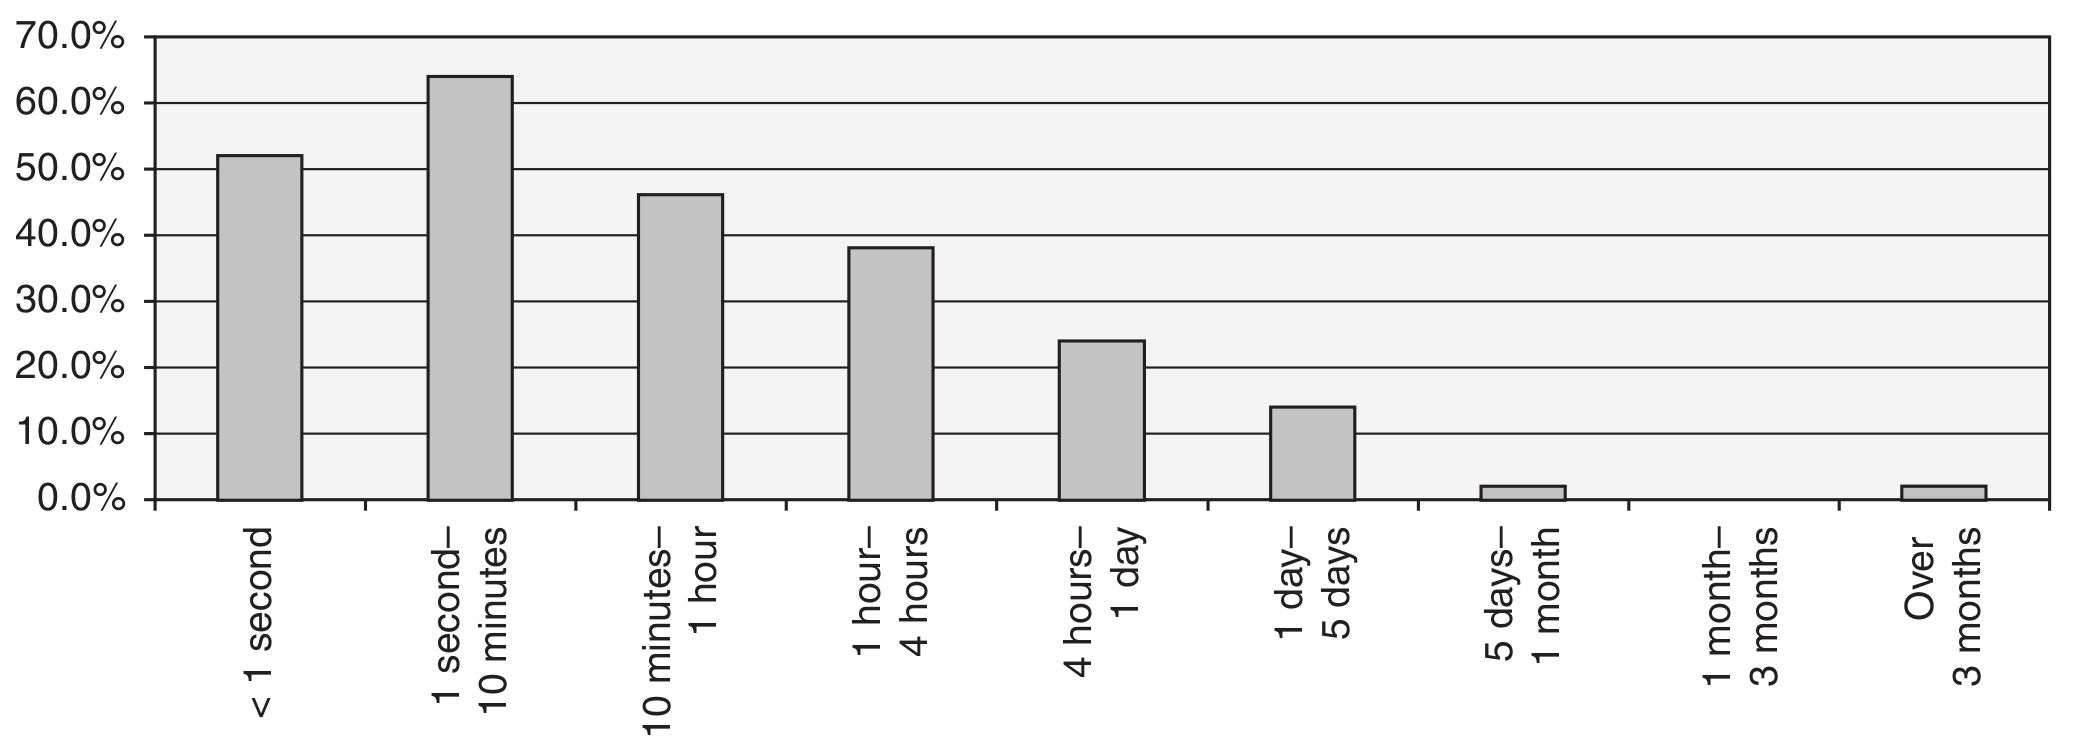
\includegraphics[width=\textwidth]{img/HFTtradestime}
  \caption{Holding time of an opened position of a high frequency trade.}
  \label{fig:HFTtimes}
\end{figure}




In 2014 HFT represents nearly 50\% of equity trades in the US and more than 20\%
in Europe showing a consistent fall since 2009 which was its best year. Revenues
have fallen dramatically.
Figure~\ref{fig:HFTmarket} shows HFT trades percentage of US equity shares.


One of the reasons of this fall is that exchange markets have adapted, having
now faster and more transparent and efficient market structures than before.
This has been possible due to its investment in technology enhancing
reliability and stability of transactions of transactions.
Even though this fall, HFT is still a major component of regulated markets and
will probably remain a topic of interest for researchers in the near future.


\begin{figure}[!h]
  %\vspace{-0.8cm}
  \centering
  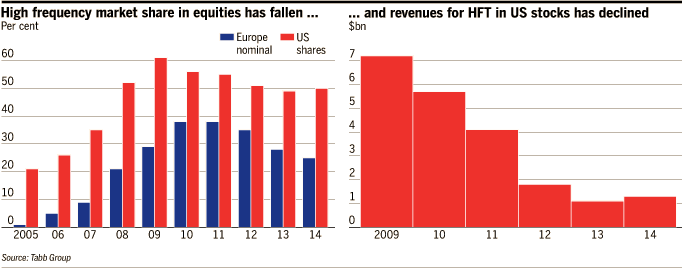
\includegraphics[width=\textwidth]{img/HFTmarket}
  \caption{Left figure shows HFT market share in the US and Europe. Right figure
  shows revenue in the US.}
  \label{fig:HFTmarket}
\end{figure}

Despite the fact HFT has been criticized on qualitative issues concerning
fairness and systemic risk, empirical research shows that HFT has lead to
beneficial impacts such as reducing spreads (difference between buyers and
sellers prices), increased liquidity, allowing more efficient price formation,
reduced transaction costs and lower market volatility.


\subsection{Financial Markets}

A financial market is any marketplace where buyers and sellers participate
trading different assets such as equities, bonds, currencies and derivatives
(future or options). One of the main objectives of financial markets is to set
prices for global trade.
A financial market has many components but the most commonly used are money
markets and capital markets. Money markets are used for short-term basis,
usually for assets up to one year, for greater periods capital markets are used.
Capital markets include the stock or equity market and the bond or debt market
and it their movements are the most widely followed.



\begin{figure}[!h]
  %\vspace{-0.8cm}
  \centering
  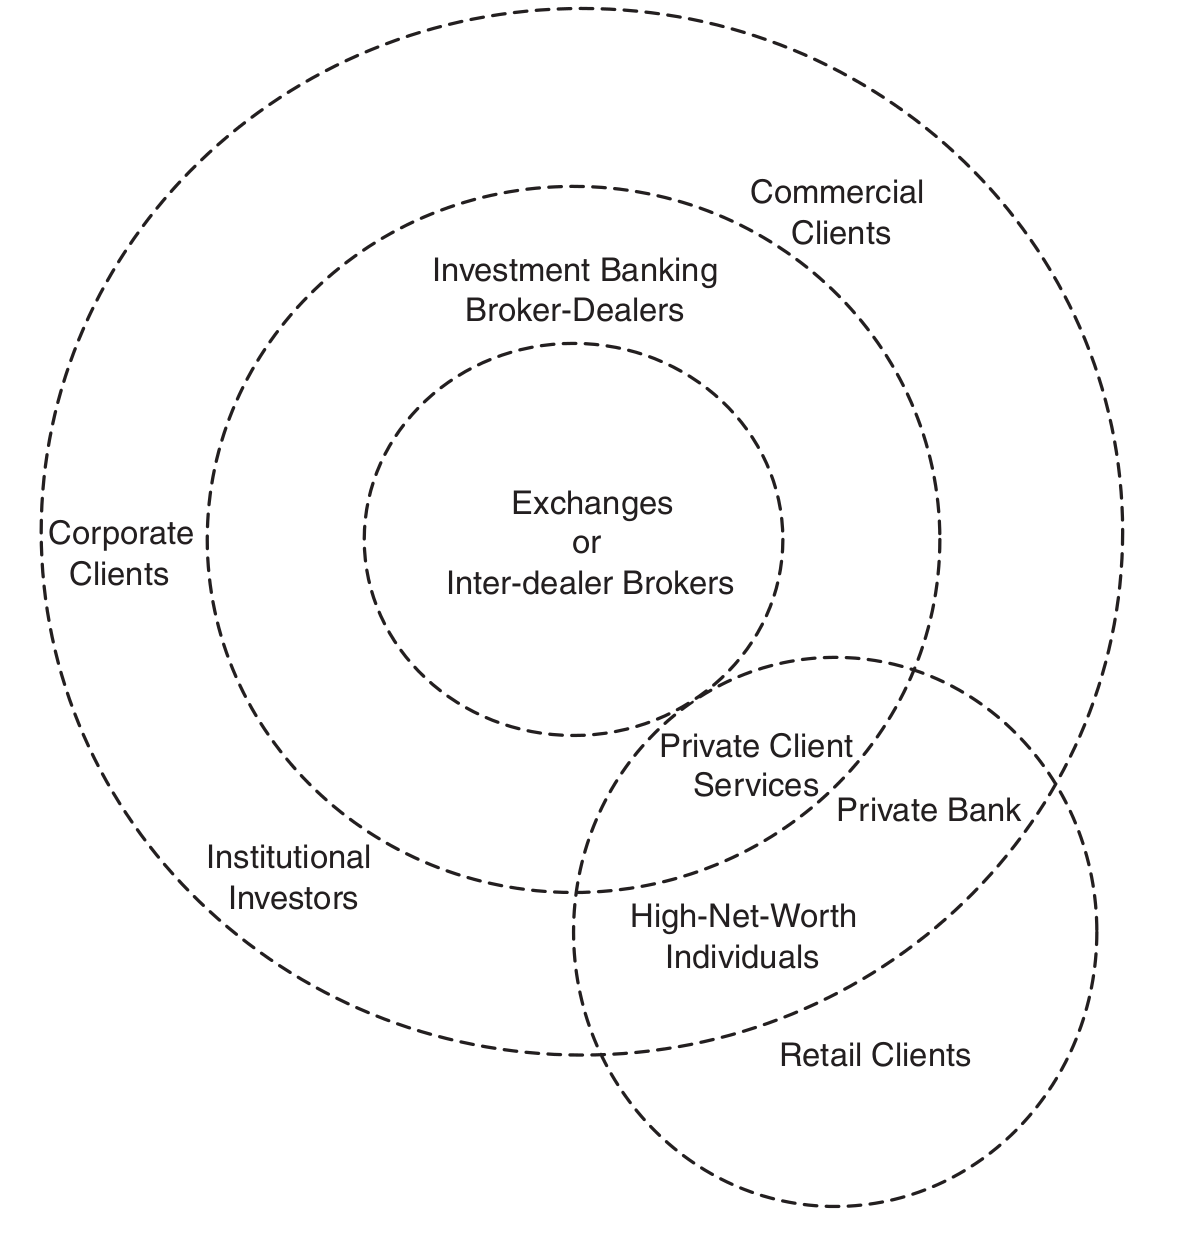
\includegraphics[width=0.7\textwidth]{img/capitalmarkets}
  \caption{Old structure of capital markets.}
  \label{fig:capitalmarket}
\end{figure}


Figure~\ref{fig:capitalmarket} shows the typical structure of capital markets
existed from the early 1929s through much of the 1990s where the broker-dealers
played the central and most profitable role.  At the core are the exchanges or
inter-dealer networks (foreign exchange trading). Exchanges are the centralized
marketplaces for transacting.  Broker-dealers perform two functions: trading for
their own accounts and transacting for their customers. Broker-dealers use
inter-dealer brokers to quickly find the best price for a particular asset among
the network of other broker-dealers. Occasionally, broker-dealers also deal
directly with other broker-dealers, particularly for less liquid instruments.
Broker-dealers clients are institutional investors, corporate clients,
commercial clients, and high-net-worth individuals.



This centralized structure existed until computer technology allowed a better
communication structure. Today financial markets are more descentralized
providing more liquidity. Exchanges and inter-dealer brokers were replaced by
liquidity pools or Electronic Communication Networks (ECNs) which are able to
transmit order quickly matching buyers and sellers optimally. There are also
dark liquidity pools where trader identity and orders remain anonymous.

Figure~\ref{fig:capitalmarketnow} shows current structucture of capital markets
including ECNs and darl pools. In this structure, ECNs, Exchanges, dark pools,
broker-dealers and retail brokerages can execute orders. However, there are some
institutional clients have also become broke-dealers.

\begin{figure}[!h]
  %\vspace{-0.8cm}
  \centering
  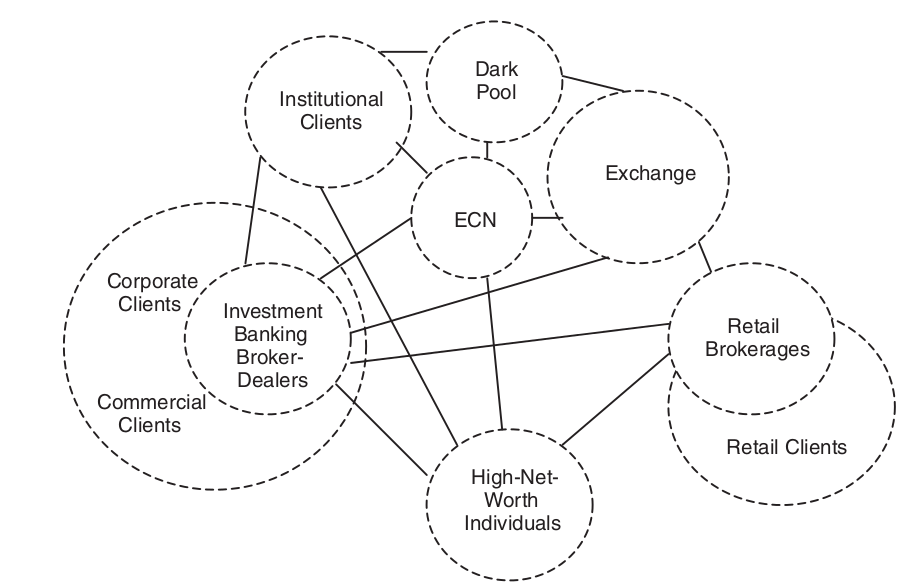
\includegraphics[width=0.8\textwidth]{img/capitalmarketsnow}
  \caption{Actual structure of capital markets.}
  \label{fig:capitalmarketnow}
\end{figure}



Equity market and foreign exchange market (Forex) are the most populat markets
for high frequency trading strategies. In equity markets can be traded stocks
such as futures and options, exchange-traded funds (ETFs) among others financial
instruments.

Forex market allows the trading of interest rates denominated pair currencies
such as EURUSD or USDJPY. Traders of this market are diverse, some of them are
high frequency traders, long-term investors and corporations. The Forex market
used to be centralized, only commercial banks had exclusive access to
inter-dealer networks. Today, Forex market is descentralized and has become the
biggest market in terms of volume of trading. The main participants are
international banks geographically dispersed with continuous 24 hours operations
excepting weekends. Figure~\ref{fig:Forextimes} shows different market trading
hours in GMT for London, New York, Sydney and Tokyo.

\begin{figure}[!h]
  %\vspace{-0.8cm}
  \centering
  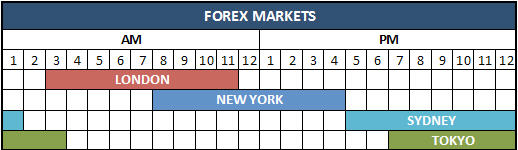
\includegraphics[width=0.8\textwidth]{img/forex-trading-hours}
  \caption{Forex market trading hours (GMT).}
  \label{fig:Forextimes}
\end{figure}

\subsection{Price formation process}


\subsection{Efficient market hypothesis}


